\section{A look at Camille}
Here are some plots;

\begin{figure}[htbp] %  figure placement: here, top, bottom, or page
   \centering
   \includegraphics[ ]{pdf/"ch 06"/"Camille intensity"} \\[25pt]
   \includegraphics[ ]{pdf/"ch 06"/"Camille sigma"} 
   \caption[Characterizing the image]{Characterizing the image of Camille Jordan. On the top we see the intensity distribution for every pixel. The brightest pixels have intensity 1; the darkest intensity 0. Below that we see the singular value spectrum for the 266 singular values. }
   \label{fig:CamilleCharacterization}
\end{figure}

In this section we wish to extend the standard presentation of image compression using the SVD.

Let's apply these procedures to a a photograph. The sample here is one of the father's of the SVD, Camille Jordan.

The matrix dimensions are these:
\begin{equation}
  \begin{array}{ccccc}
    \A{}          & = & \Y{} & \sig{} & \X{T} \\
    \by{326}{266} & = & \by{326}{326} & \by{326}{266} & \by{266}{266}
  \end{array}
\end{equation}

How much information is needed to store the picture as an array of reals? A total of 86,716 ( = 326 $\times$ 266 ) reals are needed.
How much information is needed to store the picture in SVD form? Here we would use the thin SVD, and

Call the total data volume $V(k)$.
\begin{table}[htdp]
\begin{center}
\begin{tabular}{lcl}
Source & dimensions & total \\
$\Y{}$ & $\by{326}{k}$ & $326k$\\
$\sig{}$ & $\by{k}{1}$ & $k$\\
$\X{}$ & $\by{266}{k}$ & $266k$\\\hline
Sum && $593k$
\end{tabular}
\end{center}
\label{tab:jordan:reals}
\caption[The census of numbers in an SVD]{The census of numbers in an SVD.}
\end{table}%

In full form, $V(266) = 593\times266 = 157,738$, an extra burden of over 80\%. The break even point is when we include the first $k=146$ singular values.

\clearpage
\break

\begin{table}[htdp]
\begin{center}
\begin{tabular}{ccc}
 & reconstituted image & error \\
 & $\hat{\A{}}$ & $\A{} - \hat{\A{}}$ \\
266 & \includegraphics[ width = 1.75in ]{pdf/fourier/Jordan_0266} & \includegraphics[ width = 1.75in ]{pdf/fourier/Jordan_diff_0266} \\
265 & \includegraphics[ width = 1.75in ]{pdf/fourier/Jordan_0265} & \includegraphics[ width = 1.75in ]{pdf/fourier/Jordan_diff_0265}\\
260 & \includegraphics[ width = 1.75in ]{pdf/fourier/Jordan_0260} & \includegraphics[ width = 1.75in ]{pdf/fourier/Jordan_diff_0260}\\
\end{tabular}
\end{center}
\label{default}
\caption[Subtract from the bottom]{Subtract from the bottom. Notice the error using almost all of the singular values. The picture contents 266 singular values.}
\end{table}%
%%%
\begin{table}[htdp]
\begin{center}
\begin{tabular}{ccc}
 & reconstituted image & error \\
 & $\hat{\A{}}$ & $\A{} - \hat{\A{}}$ \\
 15 & \includegraphics[ width = 1.75in ]{pdf/fourier/Jordan_0015} & \includegraphics[ width = 1.75in ]{pdf/fourier/Jordan_diff_0015} \\
 10 & \includegraphics[ width = 1.75in ]{pdf/fourier/Jordan_0010} & \includegraphics[ width = 1.75in ]{pdf/fourier/Jordan_diff_0010}\\
  5 & \includegraphics[ width = 1.75in ]{pdf/fourier/Jordan_0005} & \includegraphics[ width = 1.75in ]{pdf/fourier/Jordan_diff_0005}\\
\end{tabular}
\end{center}
\label{default}
\caption[Add from the top]{Add from the top. A surprisingly small number of singular values are able to convey most of the image information. Both the decomposition and the error contains a quality image also.}
\end{table}%
%%%
\begin{table}[htdp]
\begin{center}
\begin{tabular}{ccc}
 & reconstituted image & error \\
 & $\hat{\A{}}$ & $\A{} - \hat{\A{}}$ \\
  3 & \includegraphics[ width = 1.75in ]{pdf/fourier/Jordan_0003} & \includegraphics[ width = 1.75in ]{pdf/fourier/Jordan_diff_0003} \\
  2 & \includegraphics[ width = 1.75in ]{pdf/fourier/Jordan_0002} & \includegraphics[ width = 1.75in ]{pdf/fourier/Jordan_diff_0002}\\
  1 & \includegraphics[ width = 1.75in ]{pdf/fourier/Jordan_0001} & \includegraphics[ width = 1.75in ]{pdf/fourier/Jordan_diff_0001}\\
\end{tabular}
\end{center}
\label{default}
\caption[Add from the top]{Add from the top. A surprisingly small number of singular values are able to convey most of the image information. Most of the image information is in the error.}
\end{table}%

\endinput

%%%
\subsection{A look at Camille Jordan}
We really have a knack for faces.

The singular values are all set to unity
\begin{equation}
  \sig{} = \mat{c}{\I{470}\\\zero}.
\end{equation}
\begin{equation}
  \sig{-1} = \mat{cc}{\I{470}&\zero}.
\end{equation}


\begin{figure}[htbp] %  figure placement: here, top, bottom, or page
   \centering
   \includegraphics[ width = 3.71248in ]{pdf/fourier/Jordan_shadow} \\[5pt]
   $\A{} = \Y{} \mat{c}{\I{470}\\\zero} \X{T}$
   \caption{Replace the singular values spectrum with units. }
   \label{fig:fourier:Hilbert:unit}
\end{figure}

\begin{figure}[htbp] %  figure placement: here, top, bottom, or page
   \centering
   \includegraphics[  width = 5in  ]{pdf/fourier/Jordan_shadow_pi}  \\[5pt]
   $\A{T} = \X{} \mat{cc}{\I{470} & \zero} \Y{T}$
   \caption[The inverse is readily available and is the transpose]{The inverse is readily available and is the transpose. $\A{} = \X{} \Y{T}$}
   \label{fig:fourier:Hilbert:pi}
\end{figure}

\clearpage

%%%
\subsection{Convolution}
\begin{table}[htdp]
\begin{center}
\begin{tabular}{ccccc}
&
\includegraphics[ width = 1.15in ]{pdf/fourier/convolution/kernel_box} & 
\includegraphics[ width = 1.15in ]{pdf/fourier/convolution/kernel_disk} &
\includegraphics[ width = 1.15in ]{pdf/fourier/convolution/kernel_diamond} & 
\includegraphics[ width = 1.15in ]{pdf/fourier/convolution/kernel_cross} \\ [5pt] 
%%
1 &
\includegraphics[ width = 1.15in ]{pdf/fourier/convolution/box_001} & 
\includegraphics[ width = 1.15in ]{pdf/fourier/convolution/disk_001} &
\includegraphics[ width = 1.15in ]{pdf/fourier/convolution/diamond_001} & 
\includegraphics[ width = 1.15in ]{pdf/fourier/convolution/cross_001} \\ [5pt] 
%%
16 &
\includegraphics[ width = 1.15in ]{pdf/fourier/convolution/box_016} & 
\includegraphics[ width = 1.15in ]{pdf/fourier/convolution/disk_016} &
\includegraphics[ width = 1.15in ]{pdf/fourier/convolution/diamond_016} & 
\includegraphics[ width = 1.15in ]{pdf/fourier/convolution/cross_016} \\ [5pt] 
%%
31 &
\includegraphics[ width = 1.15in ]{pdf/fourier/convolution/box_031} & 
\includegraphics[ width = 1.15in ]{pdf/fourier/convolution/disk_031} & 
\includegraphics[ width = 1.15in ]{pdf/fourier/convolution/diamond_031} & 
\includegraphics[ width = 1.15in ]{pdf/fourier/convolution/cross_031} \\ [5pt]
%%
46 &
\includegraphics[ width = 1.15in ]{pdf/fourier/convolution/box_046} & 
\includegraphics[ width = 1.15in ]{pdf/fourier/convolution/disk_046} &
\includegraphics[ width = 1.15in ]{pdf/fourier/convolution/diamond_046} & 
\includegraphics[ width = 1.15in ]{pdf/fourier/convolution/cross_046} \\ [5pt] 
\end{tabular}
\end{center}
\label{default}
\caption{default}
\end{table}%

\clearpage
\begin{landscape}
\thispagestyle{empty}
\begin{table}[htdp]
\begin{center}
\begin{tabular}{cc}
\includegraphics[ width = 3.75in ]{pdf/fourier/convolution/box_sigma} & \qquad
\includegraphics[ width = 3.75in ]{pdf/fourier/convolution/disk_sigma} \\[15pt]
\includegraphics[ width = 3.75in ]{pdf/fourier/convolution/diamond_sigma} & \qquad
\includegraphics[ width = 3.75in ]{pdf/fourier/convolution/cross_sigma} \\[5pt]
\end{tabular}
\end{center}
\label{default}
\caption{Convolution operations.}
\end{table}%
\end{landscape}

%%%
\subsection{Shifting columns and rows}
\begin{equation}
  \begin{split}
    \Y{} & = \mat{c|c|c|c}{y_{1} & y_{2} & \dots & y_{n}}\\
    \Y{}_{s} & = \mat{c|c|c|c|c|c|c|c}{y_{s+1} & y_{s+2} & \dots & y_{n} & y_{1} & y_{2} & \dots & y_{s}}\\    
  \end{split}
\end{equation}
%%
\begin{equation}
  \A{} = \Y{}\,\sig{}\,\mat{c|c}{\X{}_{*,151-n} & \X{}_{*,1-150}}^{\mathrm{T}}
\end{equation}

\begin{figure}[htbp] %  figure placement: here, top, bottom, or page
   \centering
   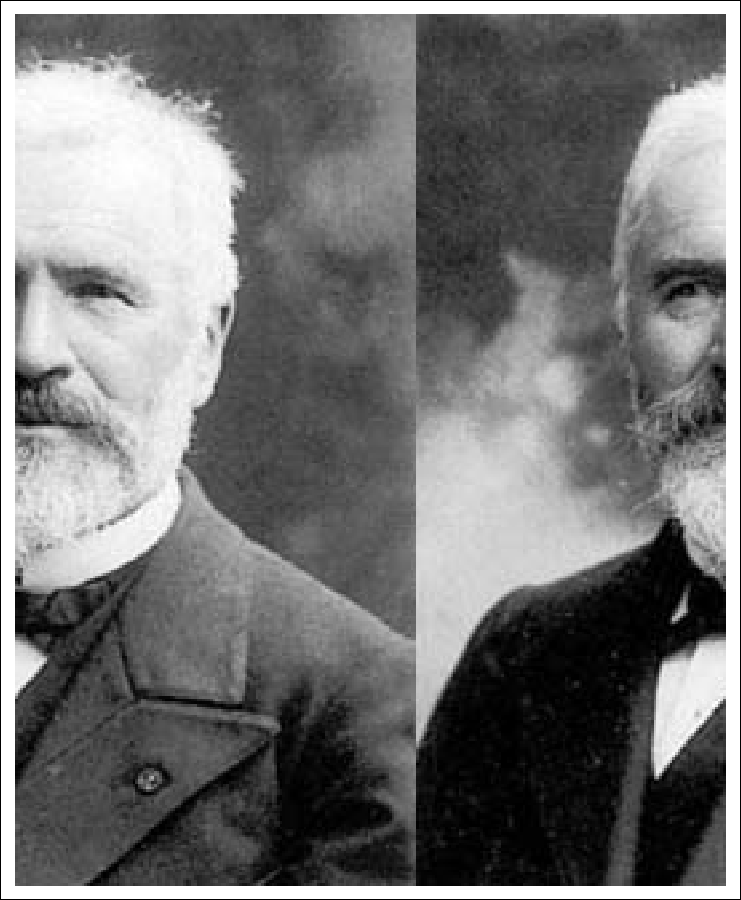
\includegraphics[ width = 2in ]{pdf/fourier/Jordan/shifts/shift_rotate_X_150} 
   \caption{}
   \label{fig:example}
\end{figure}
\clearpage

\begin{landscape}
\thispagestyle{empty}
\begin{table}[htdp]
\begin{center}
\begin{tabular}{ccc}
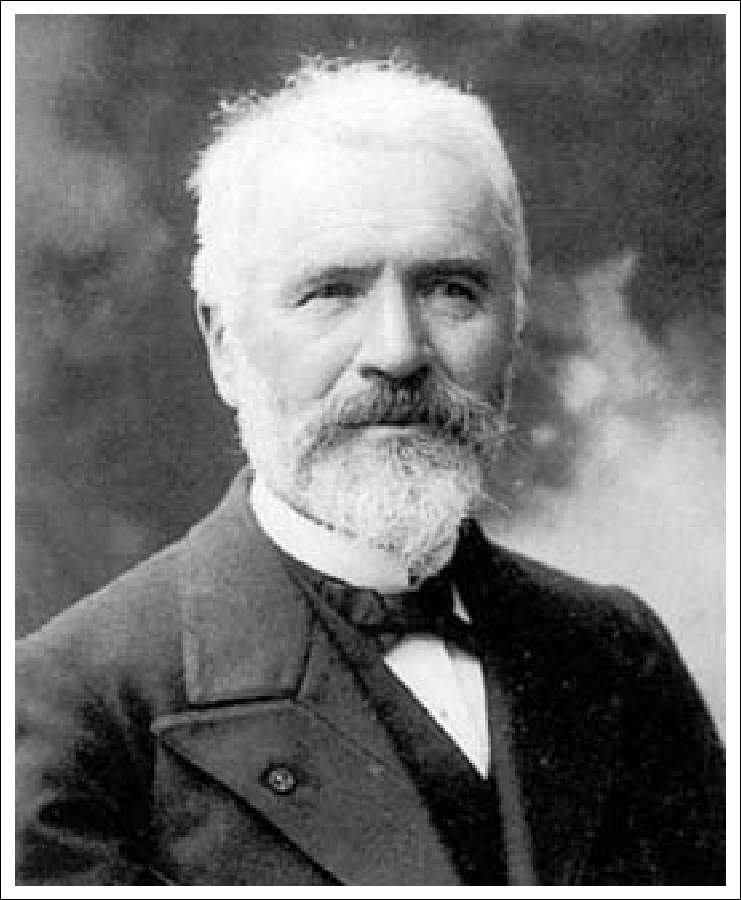
\includegraphics[ width = 2.75in ]{pdf/fourier/Jordan/shifts/shifts_good_X} &
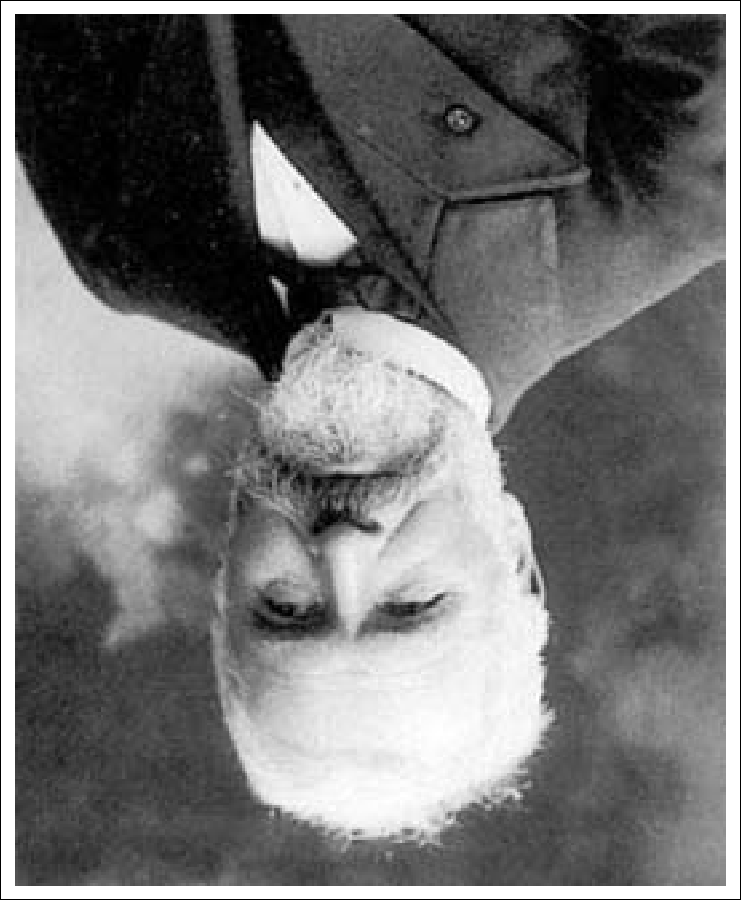
\includegraphics[ width = 2.75in ]{pdf/fourier/Jordan/shifts/shifts_good_Y} &
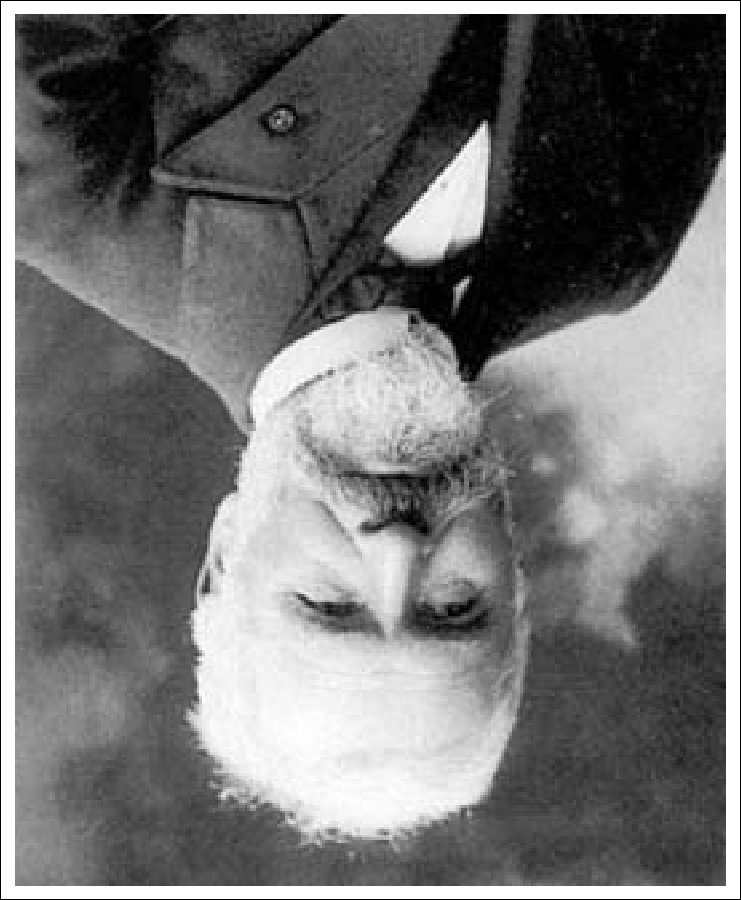
\includegraphics[ width = 2.75in ]{pdf/fourier/Jordan/shifts/shifts_good_X_Y} \\
$\A{}=\Y{}\,\sig{}\,\paren{\K{n}\X{}}^{\mathrm{T}}$ &
$\A{}=\paren{\K{m}\Y{}}\,\sig{}\,\X{T}$ &
$\A{}=\paren{\K{m}\Y{}}\,\sig{}\,\paren{\K{n}\X{}}^{\mathrm{T}}$ \\
$\dots$ &
$\dots$ &
$\dots$ \\
reverse rows in $\X{}$ &
reverse rows in $\Y{}$ &
reverse rows in $\X{}$ and $\Y{}$\\[5pt]
right-left flip &
up-down flip &
right-left, up-down flip\\[5pt]
\end{tabular}
\end{center}
\label{default}
\caption{Complete row shifts are valid operations.}
\end{table}%

\clearpage
\thispagestyle{empty}
\begin{table}[htdp]
\begin{center}
\begin{tabular}{ccc}
\includegraphics[ width = 2.75in ]{pdf/fourier/Jordan/shifts/shifts_bad_X} &
\includegraphics[ width = 2.75in ]{pdf/fourier/Jordan/shifts/shifts_bad_Y} &
\includegraphics[ width = 2.75in ]{pdf/fourier/Jordan/shifts/shifts_bad_X_Y} \\
$\A{}=\Y{}\,\sig{}\,\paren{\X{}\K{n}}^{\mathrm{T}}$ &
$\A{}=\paren{\Y{}\K{m}}\,\sig{}\,\X{T}$ &
$\A{}=\paren{\Y{}\K{m}}\,\sig{}\,\paren{\X{}\K{n}}^{\mathrm{T}}$ \\
$\dots$ &
$\dots$ &
$\dots$ \\
reverse columns in $\X{}$ &
reverse columns in $\Y{}$ &
reverse columns in $\X{}$ and $\Y{}$\\[5pt]
\end{tabular}
\end{center}
\label{default}
\caption{Complete column shifts are invalid operations. A few representative operations show that complete row shifts destroy the image information.}
\end{table}%

\clearpage
\thispagestyle{empty}
\begin{table}[htdp]
\begin{center}
\begin{tabular}{ccc}
\includegraphics[ width = 2.75in ]{pdf/fourier/Jordan/shifts/shift_rotate_X_150} &
\includegraphics[ width = 2.75in ]{pdf/fourier/Jordan/shifts/shift_rotate_Y_200} &
\includegraphics[ width = 2.75in ]{pdf/fourier/Jordan/shifts/shift_rotate_Y_200_X_150} \\
$\X{} \quad \to \quad \mat{c}{\X{}_{*,151-n} \\\hline \X{}_{*,1-150}}$ &
$\Y{} \to \mat{c}{\Y{}_{*,201-m} \\\hline \Y{}_{*,1-200}}$ &
$\X{} \to \mat{c}{\X{}_{*,151-n} \\\hline \X{}_{*,1-150}}$ \\ &&
$\Y{} \to \mat{c}{\Y{}_{*,201-m} \\\hline \Y{}_{*,1-200}}$ \\[10pt]
\end{tabular}
\end{center}
\label{default}
\caption{Shifting column vectors. When the column vectors of the domain matrix $\X{}$ are pushed to the right, the image moves to the right. Here the shift is 150 columns. When the column vectors of the codomain matrix $\Y{}$ are pushed to the right, the image moves up. The moves are independent as shown in the third image where both domain matrices are shifted.}
\end{table}%
\end{landscape}

%%%
\subsection{Block operations}
\clearpage
\break
\begin{equation*}
  \begin{split}
    \mathbb{A} & =
    \mat{ccccc}{ \Y{} & \Y{} & \Y{} & \Y{} & \Y{} \\ \Y{} & \Y{} & \Y{} & \Y{} & \Y{} \\ \Y{} & \Y{} & \Y{} & \Y{} & \Y{} \\ \Y{} & \Y{} & \Y{} & \Y{} & \Y{} \\ \Y{} & \Y{} & \Y{} & \Y{} & \Y{} } \,
    \mat{ccccc}{ \sig{} & \sig{} & \sig{} & \sig{} & \sig{} \\ \sig{} & \sig{} & \sig{} & \sig{} & \sig{} \\ \sig{} & \sig{} & \sig{} & \sig{} & \sig{} \\ \sig{} & \sig{} & \sig{} & \sig{} & \sig{} \\ \sig{} & \sig{} & \sig{} & \sig{} & \sig{} } \,
    \mat{ccccc}{ \X{} & \X{} & \X{} & \X{} & \X{} \\ \X{} & \X{} & \X{} & \X{} & \X{} \\ \X{} & \X{} & \X{} & \X{} & \X{} \\ \X{} & \X{} & \X{} & \X{} & \X{} \\ \X{} & \X{} & \X{} & \X{} & \X{} }^{\mathrm{T}} \\
  \end{split}
\end{equation*}

\includegraphics[ ]{pdf/"ch 07"/Jordan_5_5}

\clearpage
\break

%%
%%
\begin{equation*}
  \mathbb{A} = 
  \mat{ccccc}{ \Y{} & \zero & \zero & \zero & \zero \\ \zero & \Y{} & \zero & \zero & \zero \\ \zero & \zero & \Y{} & \zero & \zero \\ \zero & \zero & \zero & \Y{} & \zero \\ \zero & \zero & \zero & \zero & \Y{} } \,
  \mat{ccccc}{ \sig{} & \zero & \zero & \zero & \zero \\ \zero & \sig{} & \zero & \zero & \zero \\ \zero & \zero & \sig{} & \zero & \zero \\ \zero & \zero & \zero & \sig{} & \zero \\ \zero & \zero & \zero & \zero & \sig{} } \,
  \mat{ccccc}{ \X{} & \zero & \zero & \zero & \zero \\ \zero & \X{} & \zero & \zero & \zero \\ \zero & \zero &\X{} &  \zero & \zero \\ \zero & \zero & \zero & \X{} & \zero \\ \zero & \zero & \zero & \zero & \X{} }^{\mathrm{T}}
\end{equation*}

\includegraphics[ ]{pdf/"ch 07"/Jordan_I_5_5}
\clearpage


\begin{equation}
  \includegraphics[ width = 1.25in ]{pdf/"ch 07"/Jordan_I_5_5_A} = 
  \includegraphics[ width = 1.25in ]{pdf/"ch 07"/Jordan_I_5_5_Y} \, 
  \includegraphics[ width = 1.25in ]{pdf/"ch 07"/Jordan_I_5_5_S} \,
  \includegraphics[ width = 1.25in ]{pdf/"ch 07"/Jordan_I_5_5_X}
\end{equation}

\begin{equation}
  \includegraphics[ width = 1.25in ]{pdf/"ch 07"/Jordan_5_5_A} = 
  \includegraphics[ width = 1.25in ]{pdf/"ch 07"/Jordan_5_5_Y} \, 
  \includegraphics[ width = 1.25in ]{pdf/"ch 07"/Jordan_5_5_S} \,
  \includegraphics[ width = 1.25in ]{pdf/"ch 07"/Jordan_5_5_X}
\end{equation}

%%%
\subsection{Block operations 2}
\clearpage
\break
\begin{equation*}
  \begin{split}
    \mathbb{A} & =
    \mat{cc}{ \Y{} & \Y{} \\ \Y{} & \Y{}} \,
    \mat{cc}{ \sig{} & \sig{} \\ \sig{} & \sig{}} \,
    \mat{cc}{ \X{} & \X{} \\ \X{} & \X{}}^{\mathrm{T}} \\
  \end{split}
\end{equation*}

\includegraphics[ ]{pdf/"ch 07"/Jordan_2_2_A}

\clearpage
\break

%%
%%
\begin{equation}
  \mathbb{A} = 
  \mat{ccccc}{ \Y{} & \zero \\ \zero & \Y{}} \,
  \mat{ccccc}{ \sig{} & \zero \\ \zero & \sig{}} \,
  \mat{ccccc}{ \X{} & \zero \\ \zero & \X{}}^{\mathrm{T}}
\end{equation}

\includegraphics[ ]{pdf/"ch 07"/Jordan_I_2_2}
\clearpage


\begin{equation}
  \includegraphics[ width = 1.25in ]{pdf/"ch 07"/Jordan_I_2_2_A} = 
  \includegraphics[ width = 1.25in ]{pdf/"ch 07"/Jordan_I_2_2_Y} \, 
  \includegraphics[ width = 1.25in ]{pdf/"ch 07"/Jordan_I_2_2_S} \,
  \includegraphics[ width = 1.25in ]{pdf/"ch 07"/Jordan_I_2_2_X}
\end{equation}

\begin{equation}
  \includegraphics[ width = 1.25in ]{pdf/"ch 07"/Jordan_2_2_A} = 
  \includegraphics[ width = 1.25in ]{pdf/"ch 07"/Jordan_2_2_Y} \, 
  \includegraphics[ width = 1.25in ]{pdf/"ch 07"/Jordan_2_2_S} \,
  \includegraphics[ width = 1.25in ]{pdf/"ch 07"/Jordan_2_2_X}
\end{equation}


\endinput